\section{Lược đồ trường hợp sử dụng (Use-case diagram)}
\subsection{Sơ đồ tổng quan}
\begin{figure}[H]
    \centering
    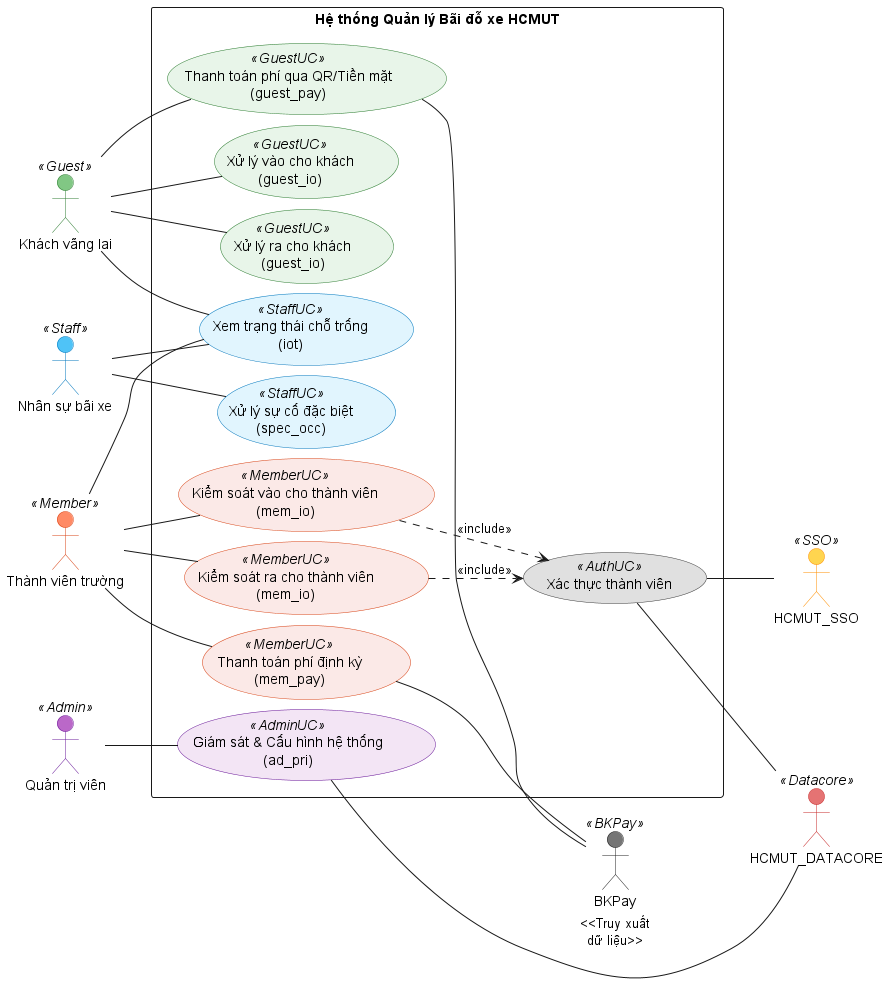
\includegraphics[width=1\linewidth]{../design/usecase-diagram/giagachad_main.png}
    \caption{Lược đồ trường hợp sử dụng tổng quát}
    \label{fig:placeholder}
\end{figure}

\subsection{Mô tả chi tiết các trường hợp sử dụng}

\subsubsection{Kiểm soát vào/ra thành viên của trường (mem\_io)}
\begingroup
\small
\begin{longtable}{|>{\centering\arraybackslash}m{3cm}|m{13.7cm}|}
\hline
\textbf{Use-case ID} & mem\_io \\ \hline
\textbf{Use-case name} & Kiểm soát vào/ra thành viên của trường \\ \hline
\textbf{Use-case overview} & Kiểm soát quá trình vào/ra của các thành viên trường (sinh viên, giảng viên, nhân viên) bằng thẻ nhận diện ID, tích hợp với cơ sở hạ tầng của trường và dịch vụ xác thực trung tâm. \\ \hline
\textbf{Actors} & Các thành viên trường HCMUT, HCMUT\_SSO (Phụ), HCMUT\_DATACORE (Phụ), Hệ thống IoT tại chỗ. \\ \hline
\textbf{Preconditions} & 
1. Hệ thống Quản lý Bãi đỗ xe Thông minh cho Khuôn viên Trường Đại học đang hoạt động và bãi đỗ còn chỗ trống. \newline
2. Thành viên thực hiện thủ tục vào/ra có thẻ nhận diện hợp lệ. \newline
3. Kết nối đến HCMUT\_SSO và HCMUT\_DATACORE phải khả dụng để xác thực theo thời gian thực. \newline
4. Thiết bị phần cứng của barrier (đầu đọc RFID, servor motor, sensors...) đang hoạt động. \\ \hline
\textbf{Trigger} & Một thành viên trường dùng thẻ nhận diện ID chạm vào đầu đọc thẻ tại cổng barrier. \\ \hline
\textbf{Steps} & 
1. Người dùng chạm thẻ nhận diện ID vào đầu đọc RFID. \newline
2. Hệ thống đọc thông tin từ thẻ nhận diện ID và xác thực người dùng thông qua dịch vụ HCMUT\_SSO. \newline
3. Hệ thống truy xuất thông tin người dùng và quyền sử dụng bãi đỗ xe của trường từ HCMUT\_DATACORE. \newline
4. Hệ thống xác thực yêu cầu thông cổng (kiểm tra hạn sử dụng của quyền sử dụng bãi đỗ xe, chống chuỗi nhập xuất bất thường như hai lần vào liên tục,...). \newline
5. Hệ thống ghi record thông cổng (ID người dùng, timestamp, ID cổng, hạn sử dụng quyền sử dụng bãi đỗ,...) trên log. \newline
6. Hệ thống cập nhật (tăng 1) tổng số lần gửi xe vào HCMUT\_DATACORE và giá trị xuất/nhập của thành viên. \newline
7. Hệ thống gửi lệnh đến servor motor controller của barrier để mở cổng. \newline
8. Cảm biến nhận diện chuyển động của phương tiện qua barrier. \newline
9. Hệ thống gửi lệnh đến servor motor controller của barrier để đóng cổng sau khi cảm biến nhận diện phương tiện đã qua cổng. \\ \hline
\textbf{Post conditions} & Quá trình thông cổng được ghi log lại, trạng thái nhập xuất của thành viên được cập nhật và cổng barrier đã đóng . \\ \hline
\textbf{Exception flow} & 
1. \textbf{Thẻ nhận diện bất hợp lệ/hết hạn:} Hệ thống từ chối thông cổng, hiện lỗi trên màn hình tại cổng, barrier tiếp tục đóng, phát cảnh báo cho nhân viên túc trực. \newline
2. \textbf{Lỗi kết nối:} Nếu không thể kết nối đến HCMUT\_SSO và HCMUT\_DATACORE, hệ thống sẽ chuyển sang sử dụng dữ liệu local và vào chế độ Manual (xử lý bởi spec\_occ). \newline
3. \textbf{Lỗi chuỗi nhập xuất bất thường:} Nếu có thành viên yêu cầu vào cổng nhưng hệ thống đã ghi nhận người này Inside (1 ví dụ trong các trường hợp lỗi này), hệ thống sẽ ghi lại log và phát cảnh báo cho nhân viên túc trực. \newline
4. \textbf{Lỗi barrier:} Nếu cảm biến barrier nhận diện có vật thể (người, phương tiện) cản trợ việc đóng cổng (barrier đang mở) thì barrier sẽ tiếp tục mở. Nếu thời gian mở hơn 15s thì sẽ phát cảnh báo. \\ \hline
\end{longtable}
\endgroup

\subsubsection{Xử lý ra/vào cho khách (guest\_io)}
\begingroup
\small
\begin{longtable}{|>{\centering\arraybackslash}m{3cm}|m{13.7cm}|}
\hline
\textbf{Use-case ID} & guest\_io \\ \hline
\textbf{Use-case name} & Xử lý ra/vào cho khách (Phát/thu thẻ xe tại chỗ) \\ \hline
\textbf{Use-case overview} & Hỗ trợ phát thẻ xe cho khách khi vào bãi và thu thẻ khi khách ra, nhằm đảm bảo việc kiểm soát phương tiện ra/vào được an toàn và chính xác. \\ \hline
\textbf{Actors} & Khách, nhân sự bãi xe, quản trị viên. \\ \hline
\textbf{Preconditions} & 
1. Hệ thống bãi xe đang hoạt động bình thường (cổng vào mở, máy phát thẻ, máy đọc thẻ và cảm biến IoT hoạt động bình thường). \newline
2. Khách vãng lai chưa có thẻ định danh trong hệ thống (không thể xác thực qua HCMUT\_SSO). \newline
3. Bãi xe còn chỗ trống. \\ \hline
\textbf{Trigger} & 
1. Khi vào bãi xe: khách nhấn nút tại máy phát thẻ $\rightarrow$ hệ thống tự động phát thẻ gửi xe. \newline
2. Khi ra khỏi bãi xe: khách đưa thẻ vào máy đọc $\rightarrow$ hệ thống tự động tính phí dựa trên thời gian gửi xe. \\ \hline
\textbf{Steps} & 
1. Khách vào nhấn nút sau đó máy phát thẻ phát thẻ gửi xe. \newline
2. Hệ thống ghi nhận thời điểm vào, ID thẻ, loại phương tiện. \newline
3. Bảng điện tử hiển thị hướng dẫn vị trí còn trống. \newline
4. Khi ra, khách đưa thẻ vào máy đọc. \newline
5. Hệ thống tra cứu phiên gửi xe, tính phí. \newline
6. Khách chọn phương thức thanh toán (Trực tuyến hoặc tiền mặt). \newline
7. Sau khi thanh toán thành công, hệ thống mở cổng cho khách ra. \newline
8. Hệ thống ghi nhận lượt ra, cập nhật trạng thái chỗ đậu. \\ \hline
\textbf{Post conditions} & 
1. Phiên gửi xe của khách được kết thúc. \newline
2. Dữ liệu gửi xe và giao dịch được lưu để phục vụ thống kê và báo cáo. \newline
3. Chỗ đậu được đánh dấu là trống. \\ \hline
\textbf{Exception flow} & 
1. Khách không nhận được thẻ khi nhấn nút (hết thẻ, lỗi kỹ thuật): 
\begin{itemize}
    \item Hệ thống hiển thị thông báo lỗi trên màn hình.
    \item Nhân sự bãi xe được cảnh báo qua hệ thống giám sát.
    \item Nhân sự cấp thẻ thủ công cho khách.
\end{itemize}
2. Khách mất thẻ gửi xe: 
\begin{itemize}
    \item Khách báo cho nhân sự bãi xe.
    \item Nhân sự tra cứu camera hoặc hệ thống để xác định thời điểm vào.
    \item Hệ thống tính phí theo chính sách “mất thẻ” (do quản trị viên cấu hình).
    \item Nhân sự cấp vé thay thế để khách ra khỏi bãi.
\end{itemize}
3. Máy đọc thẻ không nhận diện được thẻ (thẻ hỏng, máy đọc lỗi)
\begin{itemize}
    \item Hệ thống hiển thị thông báo lỗi.
    \item Nhân sự bãi xe hỗ trợ bằng cách nhập ID thẻ thủ công vào hệ thống.
    \item Nếu không thể xác định, áp dụng chính sách ngoại lệ (do quản trị viên cấu hình).
\end{itemize}
4. Cảm biến IoT báo sai trạng thái chỗ đậu (cảm biến hỏng, dữ liệu trễ):
\begin{itemize}
    \item Hệ thống đánh dấu cảm biến lỗi và loại bỏ khỏi tính toán.
    \item Nhân sự bãi xe kiểm tra thực tế và cập nhật trạng thái thủ công.
\end{itemize}
\\ \hline
\end{longtable}
\endgroup

\subsubsection{Thanh toán phí gửi xe đối với thành viên (mem\_pay)}
\begingroup
\small
\begin{longtable}{|>{\centering\arraybackslash}m{3cm}|m{13.7cm}|}
\hline
\textbf{Use-case ID} & mem\_pay \\ \hline
\textbf{Use-case name} & Thanh toán phí gửi xe đối với thành viên \\ \hline
\textbf{Use-case overview} & Hỗ trợ các thành viên trong trường thanh toán phí gửi xe định kỳ (chu kỳ 3 tháng) thông qua cổng BKPay. Phí gửi xe được tính toán tự động dựa trên tổng số phiên gửi xe (parking sessions) phát sinh trong chu kỳ đó. \\ \hline
\textbf{Actors} & Thành viên trong trường, Hệ thống BKPay (Phụ), HCMUT\_DATACORE (Phụ). \\ \hline
\textbf{Preconditions} & 
1. Hệ thống bãi xe đang hoạt động và có kết nối Internet. \newline
2. Tài khoản của thành viên đã được xác thực thông qua HCMUT\_SSO. \newline
3. Hệ thống đã tổng hợp số lượng phiên gửi xe (sessions) của thành viên trong chu kỳ 3 tháng. \newline
4. Kết nối từ hệ thống đến cổng thanh toán BKPay đang ở trạng thái khả dụng. \\ \hline
\textbf{Trigger} & Người dùng truy cập vào chức năng "Thanh toán phí gửi xe" trên hệ thống, hoặc bấm vào liên kết thanh toán từ email thông báo nhắc nhở đóng phí. \\ \hline
\textbf{Steps} & 
1. Hệ thống truy xuất dữ liệu định danh của thành viên từ HCMUT\_DATACORE và tra cứu tổng số phiên gửi xe chưa thanh toán trong chu kỳ 3 tháng vừa qua. \newline
2. Hệ thống tính toán tổng chi phí và hiển thị chi tiết hóa đơn (số lượng phiên, đơn giá, tổng tiền) trên màn hình thiết bị của người dùng. \newline
3. Người dùng kiểm tra thông tin hóa đơn và nhấn chọn "Thanh toán". \newline
4. Hệ thống tự động khởi tạo yêu cầu giao dịch và chuyển hướng người dùng sang cổng thanh toán BKPay. \newline
5. Người dùng hoàn tất các thao tác chuyển khoản/quẹt thẻ trên nền tảng BKPay. \newline
6. BKPay gửi phản hồi xác nhận giao dịch thành công về cho hệ thống. \newline
7. Hệ thống cập nhật trạng thái các phiên gửi xe trong chu kỳ thành "Đã thanh toán" và hiển thị thông báo giao dịch thành công cho người dùng. \\ \hline
\textbf{Post conditions} & Trạng thái hóa đơn chu kỳ 3 tháng của thành viên được cập nhật thành "Đã thanh toán", hệ thống lưu lại lịch sử giao dịch. \\ \hline
\textbf{Exception flow} & 
1. Mất kết nối BKPay (tại bước 4 hoặc 6): Hệ thống thông báo lỗi kết nối, yêu cầu người dùng thử lại sau và giữ nguyên trạng thái hóa đơn là "Chưa thanh toán". \newline
2. Giao dịch thất bại (không đủ số dư, người dùng hủy ngang...): Nhận phản hồi lỗi từ BKPay, hệ thống thông báo "Giao dịch thất bại" trên màn hình và ghi nhận log lỗi. \\ \hline
\end{longtable}
\endgroup

\subsubsection{Thanh toán phí gửi xe đối với khách vãng lai (guest\_pay)}
\begingroup
\small
\begin{longtable}{|>{\centering\arraybackslash}m{3cm}|m{13.7cm}|}
\hline
\textbf{Use-case ID} & guest\_pay \\ \hline
\textbf{Use-case name} & Thanh toán phí gửi xe đối với khách vãng lai \\ \hline
\textbf{Use-case overview} & Hỗ trợ khách vãng lai thanh toán phí gửi xe khi rời khỏi bãi đỗ xe trong trường. Khách có thể thanh toán qua cổng BKPay (chuyển khoản) hoặc trực tiếp bằng tiền mặt thông qua nhân sự bãi xe. \\ \hline
\textbf{Actors} & Khách vãng lai (Actor chính), Nhân sự bãi xe (Actor phụ), Hệ thống BKPay (Actor phụ), Quản trị viên (Actor phụ). \\ \hline
\textbf{Preconditions} &
1. Khách đã được phát thẻ xe tại thời điểm vào bãi. \newline
2. Hệ thống bãi xe đang hoạt động và đã ghi nhận thời gian vào của khách. \newline
3. Khách đang trong quá trình ra khỏi bãi và cần thanh toán phí gửi xe. \\ \hline
\textbf{Trigger} & Khách đã đưa thẻ vào máy đọc và hệ thống đã tra cứu phiên gửi xe, tính xong phí. \\ \hline
\textbf{Steps} &
1. Hệ thống đọc thông tin thẻ xe và tra cứu log ghi nhận thời gian vào tương ứng. \newline
2. Hệ thống tính toán phí gửi xe dựa trên khoảng thời gian gửi xe thực tế và hiển thị số tiền cần thanh toán. \newline
3. Màn hình thông báo số tiền và hỏi khách lựa chọn phương thức thanh toán: "Chuyển khoản qua BKPay" hoặc "Tiền mặt". \newline
4a. \textit{Nếu chọn chuyển khoản:} Hệ thống tạo yêu cầu thanh toán và hiển thị mã QR/thông tin BKPay cho khách. \newline
5a. Khách thực hiện chuyển khoản trên ứng dụng BKPay. \newline
6a. BKPay gửi phản hồi xác nhận giao dịch thành công về cho hệ thống. \newline
4b. \textit{Nếu chọn tiền mặt:} Khách đưa tiền mặt vào khe nhận tiền của máy tự động. \newline
5b. Hệ thống xác nhận đã thu đủ số tiền và cập nhật trạng thái thanh toán trên hệ thống. \newline
7. Hệ thống cập nhật trạng thái thẻ xe thành "Đã thanh toán", ghi log thời gian ra và mở barrier cho khách ra. \newline
8. Khách nhét thẻ xe vào khe nhận thẻ của máy tự động. \\ \hline
\textbf{Post conditions} & Phí gửi xe của khách đã được thanh toán, barrier được mở, log ghi nhận thời gian ra đầy đủ (thời gian vào - ra, biển số xe, nhân sự tại thời điểm). Thẻ xe được thu hồi và sẵn sàng tái sử dụng. \\ \hline
\textbf{Exception flow} &
1. Mất kết nối BKPay (tại bước 4a hoặc 6a): Hệ thống thông báo lỗi kết nối, nhân sự hướng dẫn khách chuyển sang thanh toán tiền mặt (chuyển sang nhánh 4b). \newline
2. Giao dịch BKPay thất bại (không đủ số dư, hủy ngang...): Nhận phản hồi lỗi từ BKPay, hệ thống thông báo "Giao dịch thất bại", hệ thống hiển thị màn hình hỗ trợ khách thử lại hoặc chuyển sang thanh toán tiền mặt. \newline
3. Khách không có tiền mặt và không thể thanh toán qua BKPay: hệ thống thông báo cho nhân sự bãi xe xử lý theo quy trình trường hợp đặc biệt (use-case spec\_occ), ghi nhận thông tin và mở barrier thủ công. \newline
4. Mất điện/mất mạng cục bộ: Hệ thống chuyển sang chế độ xử lý cục bộ, lưu log offline và nhân sự thu phí tiền mặt, đồng bộ dữ liệu lên HCMUT\_DATACORE khi kết nối được khôi phục. \\ \hline
\end{longtable}
\endgroup

\subsubsection{Quản lý nghiệp vụ hệ thống bãi xe (ad\_ops)}
\begingroup
\small
\begin{longtable}{|>{\centering\arraybackslash}m{3cm}|m{13.7cm}|}
\hline
\textbf{Use-case ID} & ad\_ops \\ \hline
\textbf{Use-case name} & Quản lý nghiệp vụ hệ thống bãi xe \\ \hline
\textbf{Use-case overview} & Cung cấp điểm truy cập tập trung để Quản trị viên (Admin) thực hiện các tác vụ quản lý, điều hành hệ thống như cấu hình tài chính, tra cứu lịch sử hoạt động. \\ \hline
\textbf{Actors} & Quản trị viên. \\ \hline
\textbf{Preconditions} & Quản trị viên đã đăng nhập vào hệ thống qua kênh xác thực HCMUT\_SSO. \\ \hline
\textbf{Trigger} & Quản trị viên truy cập vào trang quản trị (Dashboard) của hệ thống bãi xe. \\ \hline
\textbf{Steps} & 
1. Hệ thống xác thực quyền hạn của tài khoản. \newline
2. Hệ thống hiển thị giao diện Dashboard với các menu chức năng quản trị. \newline
3. Quản trị viên lựa chọn một phân hệ nghiệp vụ cụ thể (Ví dụ: "Quản lý tài chính" hoặc "Tra cứu ra vào"...). \\ \hline
\textbf{Post conditions} & Hệ thống điều hướng Quản trị viên đến đúng chức năng nghiệp vụ đã chọn để tiến hành các thao tác chi tiết. \\ \hline
\textbf{Exception flow} & 
1. Lỗi phân quyền (Xảy ra tại Bước 1): \newline
- Nếu tài khoản đăng nhập không có quyền Admin, hệ thống từ chối truy cập. \newline
- Hệ thống hiển thị thông báo "Bạn không có quyền truy cập chức năng này" và điều hướng về trang chủ. \\ \hline
\end{longtable}
\endgroup

\subsubsection{Thay đổi chi phí của 1 chu kì gửi xe (ad\_pri)}
\begingroup
\small
\begin{longtable}{|>{\centering\arraybackslash}m{3cm}|m{13.7cm}|}
\hline
\textbf{Use-case ID} & ad\_pri \\ \hline
\textbf{Use-case name} & Thay đổi chi phí của 1 chu kì gửi xe \\ \hline
\textbf{Use-case overview} & Giúp quản trị viên thay đổi các chi phí gửi xe của  chu kì gửi đối với các đối tượng nhất định như học viên, giảng viên , khách vãng lai. \\ \hline
\textbf{Actors} & Quản trị viên. \\ \hline
\textbf{Preconditions} & Quản trị viên đã đăng nhập vào hệ thống qua kênh xác thực HCMUT\_SSO \\ \hline
\textbf{Trigger} & Quản trị viên truy cập vào menu "Quản lý tài chính" trong menu "Quản trị viên" và chọn "Cấu hình chính sách giá" \\ \hline
\textbf{Steps} & 
1. Admin nhấp vào menu "Quản lý tài chính" và chọn tính năng "Cấu hình chính sách giá" trên giao diện trang quản trị. \newline
2. Hệ thống truy xuất dữ liệu và hiển thị danh sách các chính sách giá/quyền lợi hiện hành được phân loại theo từng nhóm người dùng (Người học, Cán bộ - Nhân viên, Khách tạm thời). \newline
3. Admin nhấp vào nút "Chỉnh sửa" cạnh nhóm đối tượng cần thay đổi mức phí (ví dụ: Giảng viên). \newline
4. Hệ thống hiển thị form nhập liệu chứa các thông số giá hiện tại. \newline
5. Admin nhập các thông số mức giá mới.\newline
6. Admin nhấn nút "Lưu cập nhật". \newline
7. Hệ thống hiển thị thông báo "Cập nhật chính sách giá thành công" và quay trở lại màn hình danh sách ở Bước 2.\\ \hline
\textbf{Post conditions} &  Chính sách giá mới được cập nhật thành công vào cơ sở dữ liệu và sẵn sàng áp dụng cho các chu kỳ tính toán phí tiếp theo.\\ \hline
\textbf{Exception flow} & 
1. Dữ liệu nhập vào không hợp lệ (Xảy ra tại Bước 7): \newline
- Hệ thống phát hiện dữ liệu nhập vào bị bỏ trống ở trường bắt buộc hoặc chứa ký tự không hợp lệ (ví dụ: mức phí là số âm). \newline
- Hệ thống chặn việc lưu dữ liệu, giữ nguyên các thông tin đã nhập trên form. \newline
- Hệ thống hiển thị thông báo lỗi màu đỏ ngay bên dưới trường dữ liệu bị sai: Vui lòng nhập mức giá hợp lệ (số lớn hơn hoặc bằng 0). \newline
- Kịch bản quay lại Bước 5 của luồng chính để Admin chỉnh sửa lại \newline
2. Admin hủy bỏ thao tác (Xảy ra tại bất kỳ bước nào từ Bước 3 đến Bước 5): \newline
- Admin nhấn nút Hủy bỏ hoặc nhấp vào menu khác. \newline
- Hệ thống cảnh báo nếu có dữ liệu đang nhập dở: Bạn có chắc chắn muốn rời đi? Các thay đổi chưa được lưu sẽ bị mất. \newline
- Nếu Admin chọn Đồng ý, hệ thống hủy toàn bộ phiên làm việc hiện tại và chuyển hướng theo yêu cầu của Admin, không lưu bất kỳ thay đổi nào.\\ \hline
\end{longtable}
\endgroup

\subsubsection{Xem Lịch sử Hoạt động (ad\_his)}
\begingroup
\small
\begin{longtable}{|>{\centering\arraybackslash}m{3cm}|m{13.7cm}|}
\hline
\textbf{Use-case ID} & ad\_his \\ \hline
\textbf{Use-case name} & Xem Lịch sử Hoạt động (View Parking Activity Logs) \\ \hline
\textbf{Use-case overview} & Giúp quản trị viên tra cứu, trích xuất dữ liệu về các lượt xe ra/vào bãi, tình trạng thẻ định danh, và các giao dịch phát sinh. Dữ liệu này giúp xử lý các sự cố mất xe, quên quẹt thẻ, hoặc để kiểm toán tài chính.. \\ \hline
\textbf{Actors} & Quản trị viên. \\ \hline
\textbf{Preconditions} & Quản trị viên đã đăng nhập vào hệ thống qua kênh xác thực HCMUT\_SSO \\ \hline
\textbf{Trigger} & Quản trị viên truy cập vào menu "Tra cứu ra vào" trên mục "Quản trị viên" \\ \hline
\textbf{Steps} & 
1. Admin nhấp vào menu "Tra cứu ra vào". \newline
2. Hệ thống hiển thị màn hình tra cứu với các trường bộ lọc (Filter) cơ bản và tự động load danh sách lịch sử của ngày hiện tại (Today). \newline
3. Admin nhập các tiêu chí tìm kiếm vào bộ lọc, ví dụ: Khoảng thời gian (Từ ngày - Đến ngày), mã số định danh (Mã số sinh viên/Cán bộ), vị trí cổng (Cổng 1, Cổng 2...), trạng thái (Vào bãi, Ra bãi, Cảnh báo lỗi). \newline
4. Admin nhấn nút Tìm kiếm (hoặc Áp dụng) \newline
5. Hệ thống kết nối cơ sở dữ liệu, truy xuất các bản ghi khớp với điều kiện.\newline
6. Hệ thống hiển thị kết quả dưới dạng bảng phân trang (pagination), bao gồm các thông tin: Thời gian, Mã định danh, Loại người dùng, Vị trí cổng, và Trạng thái. \newline
7. Hệ thống hiển thị thông báo "Cập nhật chính sách giá thành công" và quay trở lại màn hình danh sách ở Bước 2.\\ \hline
\textbf{Post conditions} & Quản trị viên xem được danh sách lịch sử hoạt động chính xác theo tiêu chí tìm kiếm.\\ \hline
\textbf{Exception flow} & 
1. Không tìm thấy dữ liệu (Xảy ra tại Bước 5): \newline
- Hệ thống truy vấn nhưng không có bản ghi nào khớp với tiêu chí tìm kiếm của tác nhân. \newline
- Hệ thống hiển thị thông báo trên màn hình: "Không tìm thấy lịch sử hoạt động nào phù hợp với điều kiện tìm kiếm" \newline
- Hệ thống giữ nguyên các điều kiện đã nhập ở Bước 3 để tác nhân dễ dàng điều chỉnh lại. \newline
2. Lỗi kết nối hoặc dữ liệu không nhất quán từ IoT Gateway (Xảy ra tại Bước 5): \newline
- Nếu có sự cố như mất kết nối gateway hoặc dữ liệu bị trễ, một số bản ghi ra/vào có thể bị thiếu thông tin hoặc hiển thị trạng thái Unknown (Không xác định). \newline
- Hệ thống vẫn hiển thị các bản ghi hiện có, nhưng đánh dấu cảnh báo (highlight màu vàng/đỏ) ở các dòng dữ liệu bị lỗi/thiếu để nhân viên vận hành biết và xử lý thủ công.\\ \hline
\end{longtable}
\endgroup

\subsubsection{Quản lý nhân sự và hành chính bãi đỗ xe (ad\_hr)}
\begingroup
\small
\begin{longtable}{|>{\centering\arraybackslash}m{3cm}|m{13.7cm}|}
\hline
\textbf{Use-case ID} & ad\_hr \\ \hline
\textbf{Use-case name} & Quản lý vận hành hệ thống bãi đỗ xe \\ \hline
\textbf{Use-case overview} & Hỗ trợ quản lý nhân sự vận hành bãi xe (chấm công, phân ca, đánh giá hiệu suất) và quản lý hành chính (báo cáo tài chính, hợp đồng, chính sách). \\ \hline
\textbf{Actors} & Nhân sự bãi xe, quản trị viên, hệ thống điều khiển. \\ \hline
\textbf{Preconditions} & 
1. Hệ thống quản lý nhân sự và hành chính đang hoạt động bình thường. \newline
2. Nhân sự đã được đăng ký trong hệ thống. \newline
3. Chính sách vận hành và biểu phí đã được cấu hình bởi quản trị viên. \\ \hline
\textbf{Trigger} & 
1. Nhân sự đăng nhập để chấm công và nhận ca trực. \newline
2. Quản trị viên yêu cầu xuất báo cáo hoặc cập nhật chính sách. \\ \hline
\textbf{Steps} & 
1. Nhân sự đăng nhập hệ thống để chấm công và nhận ca trực. \newline
2. Hệ thống điều khiển ghi nhận ca trực, phân ca và lưu dữ liệu nhân sự. \newline
3. Nhân sự theo dõi camera, cảm biến và tiếp nhận yêu cầu hỗ trợ từ khách. \newline
4. Hệ thống IoT thu thập dữ liệu cảm biến, phát hiện sự cố và gửi trạng thái cho hệ thống điều khiển. \newline
5. Hệ thống điều khiển quản lý hợp đồng, hồ sơ nhân sự; đồng thời thống kê lượt vào/ra và doanh thu. \newline
6. Quản trị viên truy cập hệ thống để xem báo cáo hành chính, đánh giá hiệu suất nhân sự. \newline
7. Quản trị viên cấu hình chính sách phí, ngoại lệ và phê duyệt báo cáo tài chính. \newline
8. Hệ thống điều khiển lưu trữ và áp dụng chính sách mới. \\ \hline
\textbf{Post conditions} & 
1. Dữ liệu nhân sự và hành chính được lưu trữ đầy đủ. \newline
2. Báo cáo tài chính và vận hành được xuất ra. \newline
3. Chính sách mới được áp dụng cho hệ thống. \\ \hline
\textbf{Exception flow} & 
1. Nhân sự không đăng nhập được (lỗi tài khoản, hệ thống): 
\begin{itemize}
    \item Hệ thống hiển thị thông báo lỗi.
    \item Quản trị viên hỗ trợ khôi phục tài khoản.
\end{itemize}
2. Dữ liệu cảm biến hoặc camera không khả dụng:
\begin{itemize}
    \item Hệ thống cảnh báo lỗi thiết bị.
    \item Nhân sự kiểm tra thực tế và cập nhật thủ công.
\end{itemize}
3. Báo cáo tài chính không thể xuất (lỗi hệ thống):
\begin{itemize}
    \item Hệ thống ghi log lỗi.
    \item Quản trị viên yêu cầu xuất lại sau khi khắc phục.
\end{itemize}
\\ \hline
\end{longtable}
\endgroup

\subsubsection{Quản lý quyền hạn, chi phí gửi xe và truy xuất dữ liệu (ad\_pri\_2)}
\begingroup
\small
\begin{longtable}{|>{\centering\arraybackslash}m{3cm}|m{13.7cm}|}
\hline
\textbf{Use-case ID} & ad\_pri \\ \hline
\textbf{Use-case name} & Quản lý quyền hạn, chi phí gửi xe và truy xuất dữ liệu \\ \hline
\textbf{Use-case overview} & Giúp quản trị viên thay đổi các chi phí gửi xe, truy xuất dữ liệu tức thời xe ra vào, chỉnh sửa định danh cá nhân( sinh viên, giảng viên, nhân viên ,...). \\ \hline
\textbf{Actors} & Quản trị viên \\ \hline
\textbf{Preconditions} & 
1. Hệ thống đang hoạt động và có kết nối Internet. \newline
2. Tài khoản của quản trị viên đã được xác thực thông qua HCMUT\_SSO. \newline
3. Kết nối từ hệ thống IoT đang ở trạng thái ổn hoạt động và kết nối ổn định. \\ \hline
\textbf{Trigger} & Quản trị viên truy cập vào bảng điều khiển và chọn "Chỉnh sửa" hoặc "Dữ liệu" trên giao diện của quản trị viên. \\ \hline
\textbf{Steps} & 
1. Quản trị viên truy cập vào giao diện quản lý hệ thống. \newline
2. Quản trị viên thực hiện cập nhật định danh cá nhân hoặc điều chỉnh bảng giá gửi xe (tháng/quý/năm). \newline
3. Hệ thống xác nhận và lưu các thay đổi vào cơ sở dữ liệu. \newline
4. Song song đó, hệ thống liên tục truy xuất dữ liệu từ các thiết bị IoT mỗi 1 giây/lần. \newline
5. Hệ thống xử lý và hiển thị thông tin về số lượng và sơ đồ vị trí chỗ trống lên màn hình giám sát theo thời gian thực.\\ \hline
\textbf{Post conditions} & Chi phí gửi xe hoặc định danh cá nhân đã được chỉnh sửa đúng ý quản trị viên và được lưu vào cơ sở dữ liệu. Màn hình giám sát hiển thị chính xác trạng thái chỗ trống hiện tại của bãi xe.\\ \hline
\textbf{Exception flow} & Nếu mất kết nối với wifi hoặc với hệ thống IoT sẽ hiển thị "Mất kết nối" hoặc "Mất kết nối với nhà xe" và xuất lại sơ đồ bãi xe lần cập nhật gần nhất. \\ \hline
\end{longtable}
\endgroup

\subsubsection{Kiểm soát số lượng và vị trí chỗ trống (iot\_1)}
\begingroup
\small
\begin{longtable}{|>{\centering\arraybackslash}m{3cm}|m{13.7cm}|}
\hline
\textbf{Use-case ID} & iot \\ \hline
\textbf{Use-case name} & Kiểm soát số lượng và vị trí chỗ trống 1s/ lần \\ \hline
\textbf{Use-case overview} & Hệ thống tự động thu thập dữ liệu giúp quản trị viên và người gửi biết được còn bao nhiêu chỗ trống. \\ \hline
\textbf{Actors} & Hệ thống IoT. \\ \hline
\textbf{Preconditions} & 
1. Hệ thống đang hoạt động và có kết nối Internet. \newline
2. Hệ thống IoT được cấp nguồn và kết nối với Internet. \newline
3. Sơ đồ bãi đỗ xe được thiết lập và đồng bộ với cơ sở dữ liệu. \\ \hline
\textbf{Trigger} & Bộ đếm thời gian tự động kích hoạt mỗi 1s theo chu kì. \\ \hline
\textbf{Steps} & 
1. Bộ đếm thời gian đếm đủ 1 giây và kích hoạt lệnh thu thập dữ liệu. \newline
2. Hệ thống cảm biến IoT đồng loạt gửi trạng thái hiện tại (có xe/không có xe) về máy chủ. \newline
3. Hệ thống tiếp nhận gói dữ liệu và đối chiếu với sơ đồ bãi đỗ. \newline
4. Hệ thống tính toán tổng số chỗ trống hiện tại và định vị tọa độ chính xác của các vị trí trống đó. \newline
5. Hệ thống lưu kết quả cập nhật vào cơ sở dữ liệu và đẩy dữ liệu mới lên giao diện màn hình giám sát. \\ \hline
\textbf{Post conditions} & Cơ sở dữ liệu và giao diện màn hình hiển thị chính xác trạng thái, số lượng và sơ đồ chỗ trống mới nhất ở giây hiện tại.\\ \hline
\textbf{Exception flow} & - \textbf{Lỗi một vài cảm biến:} Nếu hệ thống không nhận được tín hiệu từ một vị trí cụ thể, hệ thống đánh dấu vị trí đó là "Bảo trì/Không xác định", tiếp tục cập nhật các vị trí khác và gửi cảnh báo cho Admin.\newline
- \textbf{Mất kết nối toàn bộ:} Nếu mất mạng hoặc IoT server sập, hệ thống giữ nguyên trạng thái bãi xe ở giây cuối cùng nhận được dữ liệu và hiển thị thông báo "Mất kết nối IoT" trên màn hình. \\ \hline
\end{longtable}
\endgroup

\subsubsection{Cập nhật trạng thái bãi đỗ xe theo thời gian thực (iot\_2)}
\begingroup
\small
\begin{longtable}{|>{\centering\arraybackslash}m{3cm}|m{13.7cm}|}
\hline
\textbf{Use-case ID} & iot \\ \hline
\textbf{Use-case name} & Cập nhật trạng thái bãi đỗ xe theo thời gian thực \\ \hline
\textbf{Use-case overview} & Hệ thống tự động ghi nhận liên tục tín hiệu từ mạng lưới cảm biến IoT để cập nhật tức thời tình trạng có xe/trống, giúp duy trì cái nhìn gần thời gian thực về tình trạng chỗ đậu xe. \\ \hline
\textbf{Actors} & Hệ thống IoT (Cảm biến \& Gateway). \\ \hline
\textbf{Preconditions} & 
1. Hệ thống máy chủ đang hoạt động và sẵn sàng nhận kết nối. \newline
2. Hạ tầng IoT (Cảm biến, Gateway) được cấp nguồn, đã kết nối mạng và hoạt động ổn định. \newline
3. Sơ đồ bãi đỗ (vị trí tương ứng của từng cảm biến) đã được thiết lập trong cơ sở dữ liệu. \\ \hline
\textbf{Trigger} & Xảy ra khi có sự thay đổi trạng thái vật lý tại bãi đỗ (có xe tiến vào vị trí hoặc rời đi) khiến cảm biến bị kích hoạt, hoặc Gateway định kỳ gửi luồng dữ liệu (stream) trạng thái toàn bãi. \\ \hline
\textbf{Steps} & 
1. Cảm biến tại vị trí đỗ xe phát hiện sự thay đổi trạng thái (Trống $\rightarrow$ Có xe, hoặc Có xe $\rightarrow$ Trống) và gửi ngay gói tin về hệ thống trung tâm thông qua IoT Gateway. \newline
2. Hệ thống tiếp nhận gói tin, phân tích định danh (ID) của cảm biến để đối chiếu với sơ đồ bãi đỗ. \newline
3. Hệ thống cập nhật ngay lập tức trạng thái của vị trí tương ứng vào cơ sở dữ liệu. \newline
4. Hệ thống tính toán lại tổng số chỗ trống hiện tại. \newline
5. Hệ thống đồng bộ (push) dữ liệu mới nhất lên các bảng hiển thị điện tử ngoài bãi xe và giao diện giám sát của ban quản lý. \\ \hline
\textbf{Post conditions} & Cơ sở dữ liệu, màn hình giám sát và bảng LED điều hướng luôn phản ánh chính xác trạng thái và số lượng chỗ trống ở thời điểm hiện tại.\\ \hline
\textbf{Exception flow} & - \textbf{Lỗi cục bộ tại cảm biến/Gateway:} Nếu hệ thống phát hiện mất luồng tín hiệu hoặc nhận dữ liệu không nhất quán từ một node mạng, hệ thống tự động đánh dấu vị trí đó là "Không xác định/Bảo trì", ghi log cảnh báo cho bộ phận vận hành và vẫn tiếp tục xử lý dữ liệu từ các node khác.\newline
- \textbf{Mất kết nối toàn bộ hệ thống IoT:} Hệ thống tạm ngưng cập nhật, đóng băng trạng thái hiển thị ở thời điểm nhận gói tin cuối cùng và phát tín hiệu cảnh báo đỏ "Mất kết nối hạ tầng IoT" trên màn hình điều hành. \\ \hline
\end{longtable}
\endgroup

\subsubsection{Xử lý sự cố đặc biệt tại bãi xe (spec\_occ)}
\begingroup
\small
\begin{longtable}{|>{\centering\arraybackslash}m{3cm}|m{13.7cm}|}
\hline
\textbf{Use-case ID} & spec\_occ \\ \hline
\textbf{Use-case name} & Xử lý sự cố đặc biệt tại bãi xe  \\ \hline
\textbf{Use-case overview} & Hỗ trợ công cụ, phương thức cho nhân viên tại bãi xe xử lý thủ công các trường hợp đặc biệt xảy ra tại bãi xe   \\ \hline
\textbf{Actors} & Nhân viên bãi xe, người gửi xe  \\ \hline
\textbf{Preconditions} & Nhân viên bãi xe đã đăng nhập hệ thống và có thông báo sự cố từ hệ thống trên màn hình điều khiển hoặc thông báo từ người dùng. \\ \hline
\textbf{Trigger} & Nhân viên bãi xe truy cập vào chức năng “Xử lý sự cố tại bãi” trên giao diện của hệ thống. \\ \hline
\textbf{Steps} & 
1. Hệ thống báo động hoặc nhận được yêu cầu hỗ trợ từ người gửi xe. \newline
2. Nhân viên bãi xe kiểm tra thông vị trí trên màn hình điều khiển và xác nhận sự cố gặp phải. \newline
3. Nhân viên bãi xe truy cập vào chức năng "Xử lý sự cố tại bãi" trên màn hình điều khiển của hệ thống. \newline
4. Nhân viên chọn loại sự cố cụ thể trên màn hình điều khiển để xử lý. \\ \hline
\textbf{Post conditions} & Hệ thống ghi lại thông tin sự cố đã xảy ra. \\ \hline
\textbf{Exception flow} & 
1. Hệ thống báo động lỗi (xác nhận sai sự cố), nhân viên tắt thông báo trên màn hình. \newline
2. Đầu đọc thẻ không nhận được dữ liệu, nhân viên yêu cầu người gửi quét thẻ lại hoặc xử lý theo các trường hợp cụ thể khác. \\ \hline
\end{longtable}
\endgroup

\subsubsection{Kích hoạt chế độ khẩn cấp (spec\_occ\_1)}
\begingroup
\small
\begin{longtable}{|>{\centering\arraybackslash}m{3cm}|m{13.7cm}|}
\hline
\textbf{Use-case ID} & spec\_occ\_1   \\ \hline
\textbf{Use-case name} & Kích hoạt chế độ khẩn cấp   \\ \hline
\textbf{Use-case overview} & Chuyển trạng thái bãi xe sang chế độ mở hoàn toàn để giải tỏa các phương tiện có trong bãi nhanh nhất khi có sự cố nghiêm trọng xảy ra. \\ \hline
\textbf{Actors} & Nhân viên bãi xe, hệ thống IoT   \\ \hline
\textbf{Preconditions} & Có tín hiệu cháy nổ hoặc tình huống khẩn cấp khác cần phải giải tỏa   \\ \hline
\textbf{Trigger} & 1. Nhân viên bãi xe chọn chức năng “Kích hoạt chế độ khẩn cấp” trên màn hình điều khiển. \newline 2. Hệ thống tự kích hoạt chế độ khẩn cấp sau 10 giây khi nhận được tín hiệu khẩn cấp từ các cảm biến. \\ \hline
\textbf{Steps} & 
1. Nhân viên bãi xe chọn chức năng “Kích hoạt chế độ khẩn cấp” khi có sự cố. \newline
2. Hệ thống mở đồng loạt các barrier tại các cổng ra/vào. \newline
3. Tạm dừng quy trình xác thực và tính phí để ưu tiên lưu thông. \\ \hline
\textbf{Post conditions} & Barrier giữ trạng thái mở, hệ thống ghi lại thông tin sự cố xảy ra. \\ \hline
\textbf{Exception flow} & 1. Nếu hệ thống điều khiển không hoạt động, các barrier được mở thủ công bằng chìa khóa cơ hoặc nút nhấn vật lý tại bàn điều khiển. \newline
2. Nếu khi không có sự cố, nhưng hệ thống đã xác nhận sai và tự kích hoạt chế độ khẩn cấp, thì buộc nhân viên phải tự tắt chế độ này tại màn hình điều khiển. \\ \hline
\end{longtable}
\endgroup

\subsubsection{Giải quyết lỗi thanh toán (spec\_occ\_2)}
\begingroup
\small
\begin{longtable}{|>{\centering\arraybackslash}m{3cm}|m{13.7cm}|}
\hline
\textbf{Use-case ID} & spec\_occ\_2   \\ \hline
\textbf{Use-case name} & Giải quyết lỗi thanh toán   \\ \hline
\textbf{Use-case overview} & Xử lý trường hợp người dùng thanh toán phí gửi xe qua hệ thống BKPay không thành công   \\ \hline
\textbf{Actors} & Nhân viên bãi xe, người dùng, hệ thống BKPay  \\ \hline
\textbf{Preconditions} & 1. Người dùng quét thẻ tại cổng ra/vào nhưng hệ thống không phản hồi. \newline
2. Hệ thống BKPay báo lỗi trên màn hình điều khiển.\newline
3. Hệ thống đưa ra mã QR thanh toán không hợp lệ, người dùng không thực hiện thanh toán qua BK\_PAY được.\\ \hline
\textbf{Trigger} & Nhân viên bãi xe chọn chức năng “Lỗi thanh toán” trên màn hình điều khiển.   \\ \hline
\textbf{Steps} & 
1. Nhân viên kiểm tra lại kết nối của hệ thống bãi xe với hệ thống BKPay và yêu cầu người gửi xe quét thẻ lại. \newline
2. Nếu vẫn chưa thành công, nhân viên bãi xe chọn chức năng “Lỗi thanh toán” trên giao diện hệ thống. \newline
3. Kiểm tra lịch sử giao dịch của người dùng theo thông tin thẻ trên hệ thống BK\_PAY \newline
4. Nhân viên thực hiện ghi đè trạng thái thanh toán và hệ thống xác nhận thanh toán thành công. \newline
5. Hệ thống ra lệnh mở barrier tự động.   \\ \hline
\textbf{Post conditions} & Hệ thống ghi lại thông tin sự cố xảy ra. \\ \hline
\textbf{Exception flow} & Nếu hệ thống BK\_PAY vẫn không xác nhận được thanh toán thành công hoặc người dùng không chuyển tiền qua mã QR được, buộc phải thanh toán bằng tiền mặt. \\ \hline
\end{longtable}
\endgroup

\subsubsection{Giải quyết quên thẻ định danh (spec\_occ\_3)}
\begingroup
\small
\begin{longtable}{|>{\centering\arraybackslash}m{3cm}|m{13.7cm}|}
\hline
\textbf{Use-case ID} & spec\_occ\_3   \\ \hline
\textbf{Use-case name} & Giải quyết quên thẻ định danh   \\ \hline
\textbf{Use-case overview} & Xử lý trường hợp người dùng quên thẻ định danh (dành cho các thành viên của nhà trường)  \\ \hline
\textbf{Actors} & Nhân viên bãi xe, người dùng, HCMUT\_DATACORE   \\ \hline
\textbf{Preconditions} & Người dùng không có thẻ định danh tại cổng khi ra hoặc vào bãi xe. \\ \hline
\textbf{Trigger} & Nhân viên bãi xe chọn chức năng “Quên thẻ định danh” trên giao diện hệ thống. \\ \hline
\textbf{Steps} & 
1. Nhân viên bãi xe chọn chức năng “Quên thẻ định danh” trên giao diện hệ thống. \newline
2. Nhân viên bãi xe yêu cầu cung cấp thông tin định danh (MSSV hoặc MSCB) để xác nhận trên hệ thống HCMUT\_DATACORE. \newline
3.1 \textbf{Khi đi vào:} Hệ thống xác nhận hợp lệ, ghi nhận phiên gửi xe thành công và phát thẻ tạm thời cho người dùng. \newline
3.2 \textbf{Khi đi ra:} Người dùng thực hiện lượt đi ra như khách vãng lai nhưng không cần yêu cầu thanh toán.  \newline
4. Hệ thống ra lệnh để mở barrier tự động. \\ \hline
\textbf{Post conditions} & Hệ thống ghi lại thông tin sự cố xảy ra và thông tin phiên gửi xe gắn với thông tin người dùng trên hệ thống HCMUT\_DATACORE. \\ \hline
\textbf{Exception flow} & Nếu không có thông tin trên HCMUT\_DATACORE, hoặc có thông tin nhưng người dùng không có đăng ký dịch vụ, người dùng buộc phải sử dụng vé tạm thời hoặc thực hiện đăng ký để sử dụng dịch vụ. \\ \hline
\end{longtable}
\endgroup

\subsubsection{Giải quyết mất vé gửi xe (spec\_occ\_4)}
\begingroup
\small
\begin{longtable}{|>{\centering\arraybackslash}m{3cm}|m{13.7cm}|}
\hline
\textbf{Use-case ID} & spec\_occ\_4   \\ \hline
\textbf{Use-case name} & Giải quyết mất vé gửi xe   \\ \hline
\textbf{Use-case overview} & Xử lý trường hợp người dùng mất vé của phiên gửi xe (dành cho người dùng vãng lai và thành viên nhà trường nếu làm mất vé tạm thời khi được cấp lúc quên mang thẻ). \\ \hline
\textbf{Actors} & Nhân viên bãi xe, người dùng, HCMUT\_DATACORE   \\ \hline
\textbf{Preconditions} & Người dùng không có vé tại cổng ra/vào. \\ \hline
\textbf{Trigger} & Nhân viên bãi xe chọn chức năng “Mất vé tạm thời” trên giao diện hệ thống. \\ \hline
\textbf{Steps} & 
\begin{enumerate}[label=\arabic*., leftmargin=1.5em, nosep]
    \item Nhân viên bãi xe chọn chức năng “Mất vé tạm thời” trên giao diện hệ thống.
    \item Nhân viên xác nhận đó là thành viên nhà trường hay khách vãng lai.
    \begin{enumerate}[label=2.\arabic*., leftmargin=2em, nosep]
        \item Nếu là thành viên nhà trường, yêu cầu cung cấp thông tin (MSSV hoặc MSCB).
        \begin{enumerate}[label=2.1.\arabic*., leftmargin=2.5em, nosep]
            \item Nhân viên xác nhận đúng thông tin về phiên gửi xe từ hệ thống và yêu cầu thực hiện phí phạt làm mất thẻ.
            \item Nhân viên chọn tạo mã QR thanh toán phí phạt nếu người dùng chọn thanh toán qua BK\_PAY hoặc thu tiền mặt tại chỗ.
        \end{enumerate}
        \item Nếu là khách vãng lai, nhân viên bãi xe yêu cầu cung cấp thông tin phương tiện (biển số xe, loại xe, thời gian vào).
        \begin{enumerate}[label=2.2.\arabic*., leftmargin=2.5em, nosep]
            \item Nhân viên kiểm tra lại trên hệ thống và nhân viên xác nhận hệ thống hiển thị thông tương ứng.
            \item Nhân viên chọn tạo mã QR thanh toán phí phạt nếu người dùng chọn thanh toán qua BK\_PAY hoặc thu tiền mặt tại chỗ.
        \end{enumerate}
    \end{enumerate}
    \item Nhân viên ra lệnh để mở barrier thủ công sau khi xác nhận thanh toán phạt thành công.
\end{enumerate} \\ \hline
\textbf{Post conditions} & Hệ thống ghi lại thông tin sự cố xảy ra, thông tin về phiên gửi xe. \\ \hline
\textbf{Exception flow} & Nếu không tìm thấy dữ liệu xe vào trên hệ thống, nhân viên báo cáo quản trị viên kiểm tra camera an ninh hoặc giấy tờ xe. \\ \hline
\end{longtable}
\endgroup

\subsubsection{Giải quyết thẻ quá hạn, không thanh toán phí (spec\_occ\_5)}
\begingroup
\small
\begin{longtable}{|>{\centering\arraybackslash}m{3cm}|m{13.7cm}|}
\hline
\textbf{Use-case ID} & spec\_occ\_5   \\ \hline
\textbf{Use-case name} & Giải quyết thẻ quá hạn, không thanh toán phí   \\ \hline
\textbf{Use-case overview} & Xử lý trường hợp người dùng không thanh toán phí hoặc thẻ chưa được gia hạn chu kỳ mới. \\ \hline
\textbf{Actors} & Nhân viên bãi xe, người dùng, HCMUT\_DATACORE \\ \hline
\textbf{Preconditions} & Hệ thống thông báo thẻ quá hạn hoặc không thanh toán phí khi quét thẻ. Barrier không mở.   \\ \hline
\textbf{Trigger} & Nhân viên bãi xe chọn chức năng “Giải quyết thẻ quá hạn, không thanh toán phí” trên giao diện hệ thống. \\ \hline
\textbf{Steps} & 
1. Nhân viên bãi xe chọn chức năng “Giải quyết thẻ quá hạn, không thanh toán phí” trên giao diện hệ thống. \newline
2. Nhân viên bãi xe kiểm tra chi tiết khoản nợ trên hệ thống quản lý. \newline
3. Nhân viên hướng dẫn thanh toán qua hệ thống BKPay (thực hiện theo quy trình mem\_pay) \newline
4. Người dùng quét thẻ lại sau khi thanh toán thành công. \\ \hline
\textbf{Post conditions} & Xóa đánh dấu quá hạn hoặc nợ phí thanh toán trên thẻ định danh. \\ \hline
\textbf{Exception flow} & Nếu hệ thống mất kết nối với BKPay, nhân viên ghi nhận thủ công giao dịch và mở barrier thủ công. \\ \hline
\end{longtable}
\endgroup

\subsubsection{Mở barrier thủ công (spec\_occ\_6)}
\begingroup
\small
\begin{longtable}{|>{\centering\arraybackslash}m{3cm}|m{13.7cm}|}
\hline
\textbf{Use-case ID} & spec\_occ\_6  \\ \hline
\textbf{Use-case name} & Mở barrier thủ công   \\ \hline
\textbf{Use-case overview} & Nhân viên can thiệp mở barrier thủ công cho các trường hợp hệ thống không tự động. \\ \hline
\textbf{Actors} & Nhân viên bãi xe, hệ thống bãi xe   \\ \hline
\textbf{Preconditions} &
1. Các trường hợp ra/vào cổng đặc biệt \newline
2. Sau khi xác thực thành công của hoạt động ra, vào nhưng hệ thống không tự động mở.
\\ \hline
\textbf{Trigger} & Nhân viên chọn chức năng “Mở barrier” trên màn hình điều khiển. \\ \hline
\textbf{Steps} & 
1. Nhân viên bãi xe chọn chức năng “Mở barrier” trên giao diện hệ thống. \newline
2. Hệ thống barrier mở sau khi nhân viên xác nhận. \\ \hline
\textbf{Post conditions} & Hệ thống ghi lại thông tin sự cố và thông tin nhân viên ra lệnh mở barrier. \\ \hline
\textbf{Exception flow} & Mở bằng nút nhấn vật lý hoặc khóa cơ nếu hệ thống không xác nhận. \\ \hline
\end{longtable}
\endgroup
